% Source: Weinberg GR, physical PDF p. 321 (printed p. 298).
% Coverage: Figure 11.1, four quasi-stellar objects.
% Status: source page extracted losslessly; photographs clipped independently
%         so that all four object labels remain complete; source-reviewed.
% Uncertainties: none.

\begingroup
\renewcommand{\thefigure}{11.1}
\begin{figure}[htbp]
  \centering
  \begin{tabular}{@{}c@{\hspace{1.5em}}c@{}}
    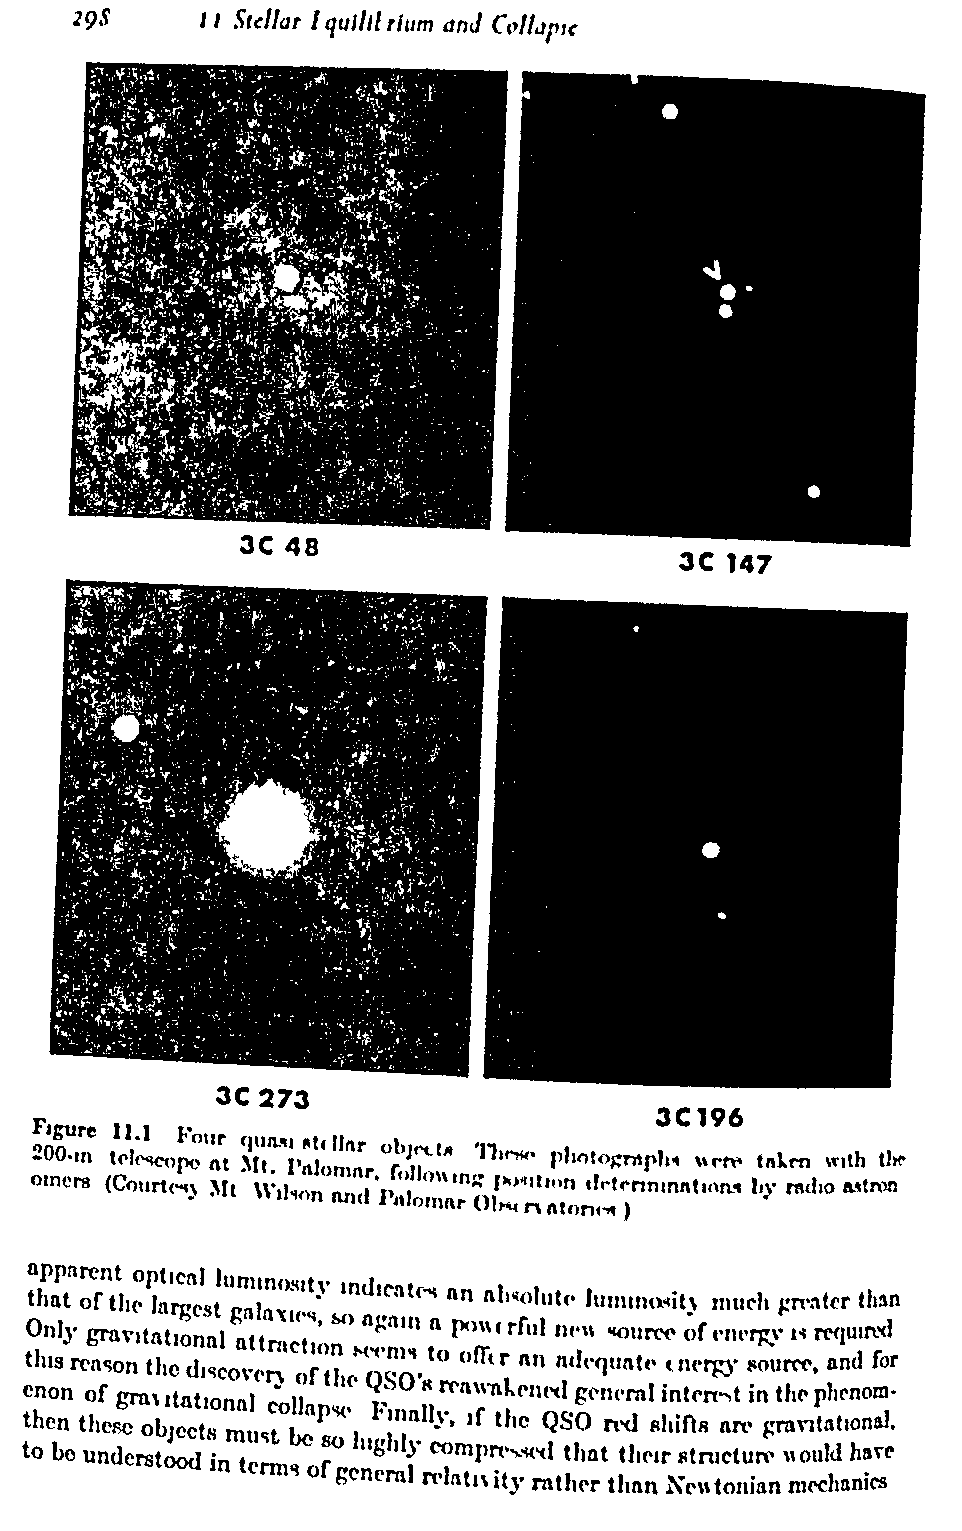
\includegraphics[
      height=0.255\textheight,
      trim=62bp 999bp 454bp 57bp,
      clip
    ]{figures/chapter11/fig11-01-source.png}
    &
    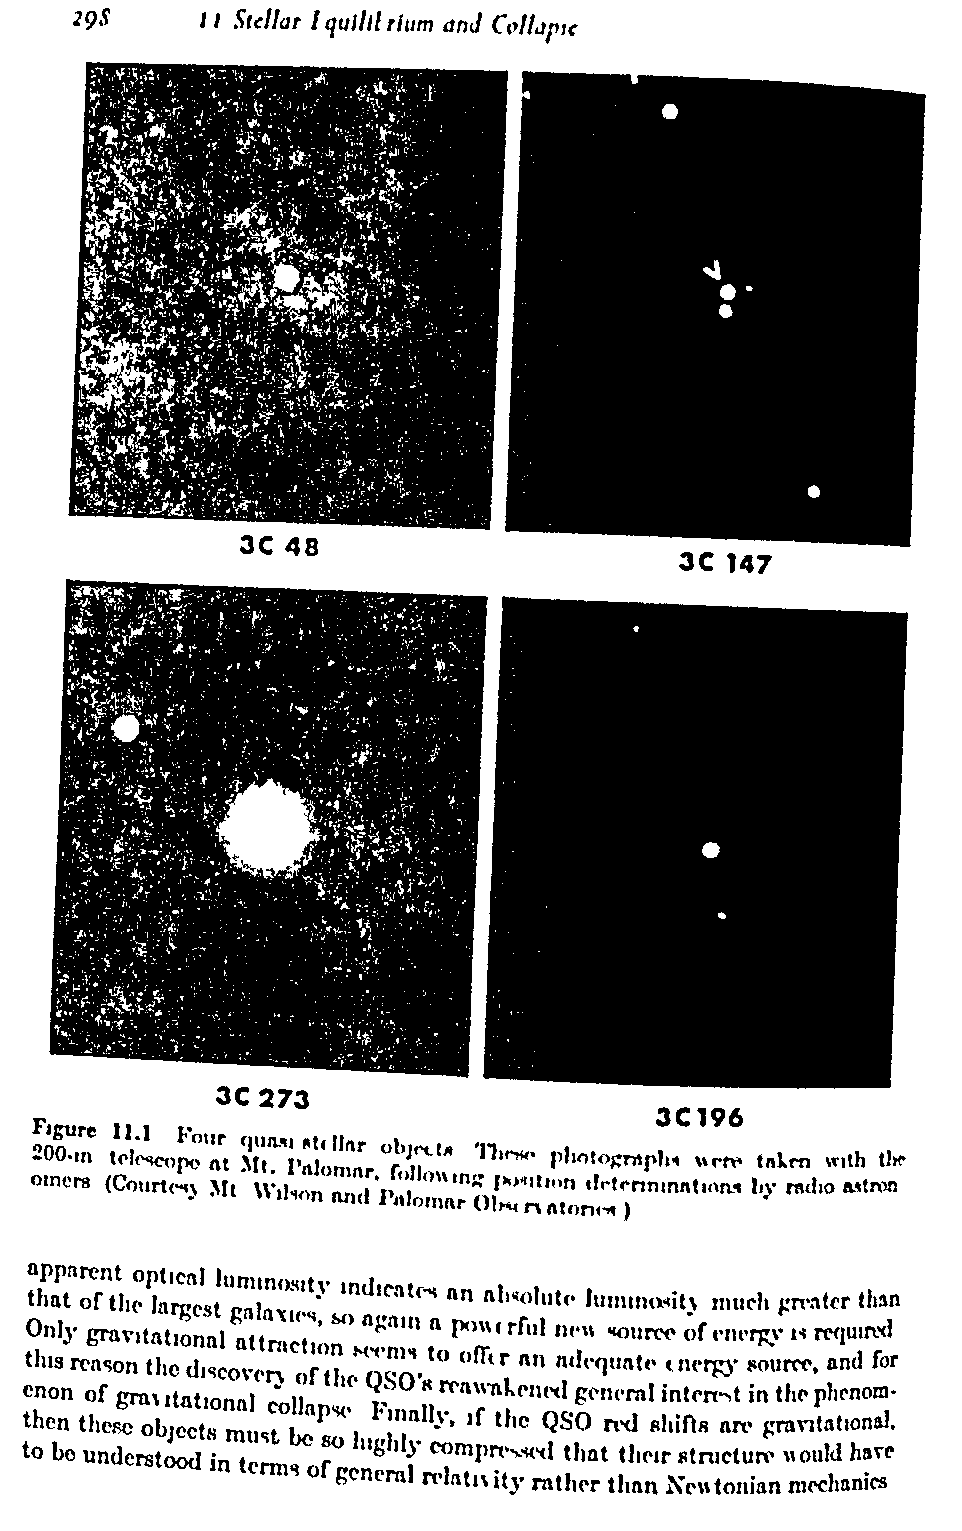
\includegraphics[
      height=0.255\textheight,
      trim=518bp 985bp 29bp 62bp,
      clip
    ]{figures/chapter11/fig11-01-source.png}
    \\
    \small\bfseries 3C 48 & \small\bfseries 3C 147
    \\[0.55em]
    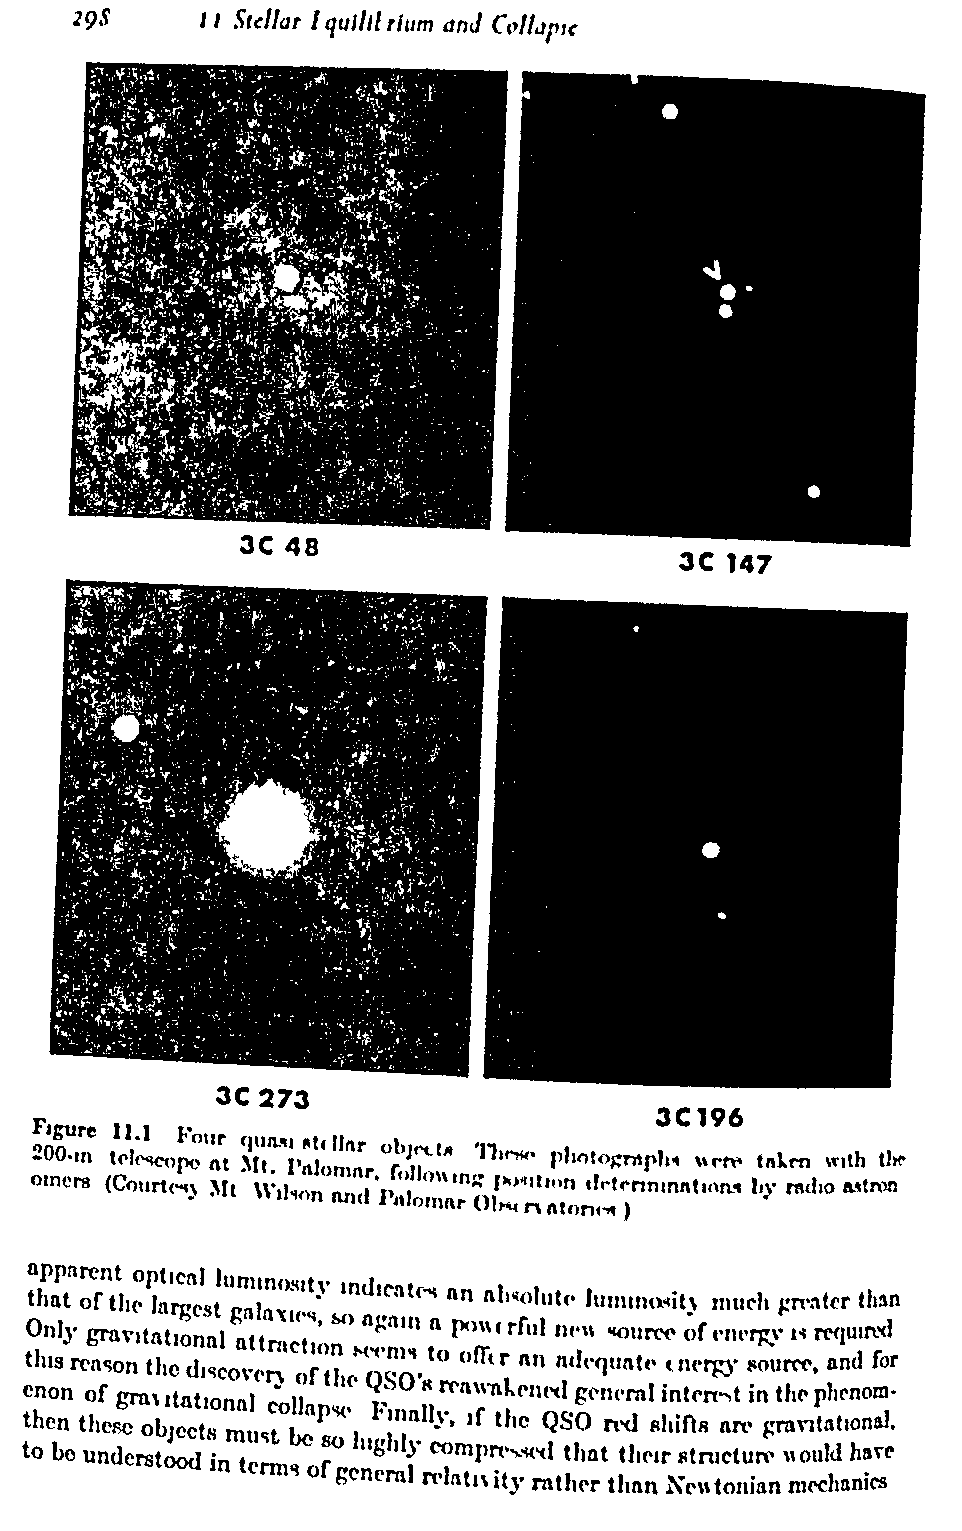
\includegraphics[
      height=0.255\textheight,
      trim=52bp 452bp 477bp 569bp,
      clip
    ]{figures/chapter11/fig11-01-source.png}
    &
    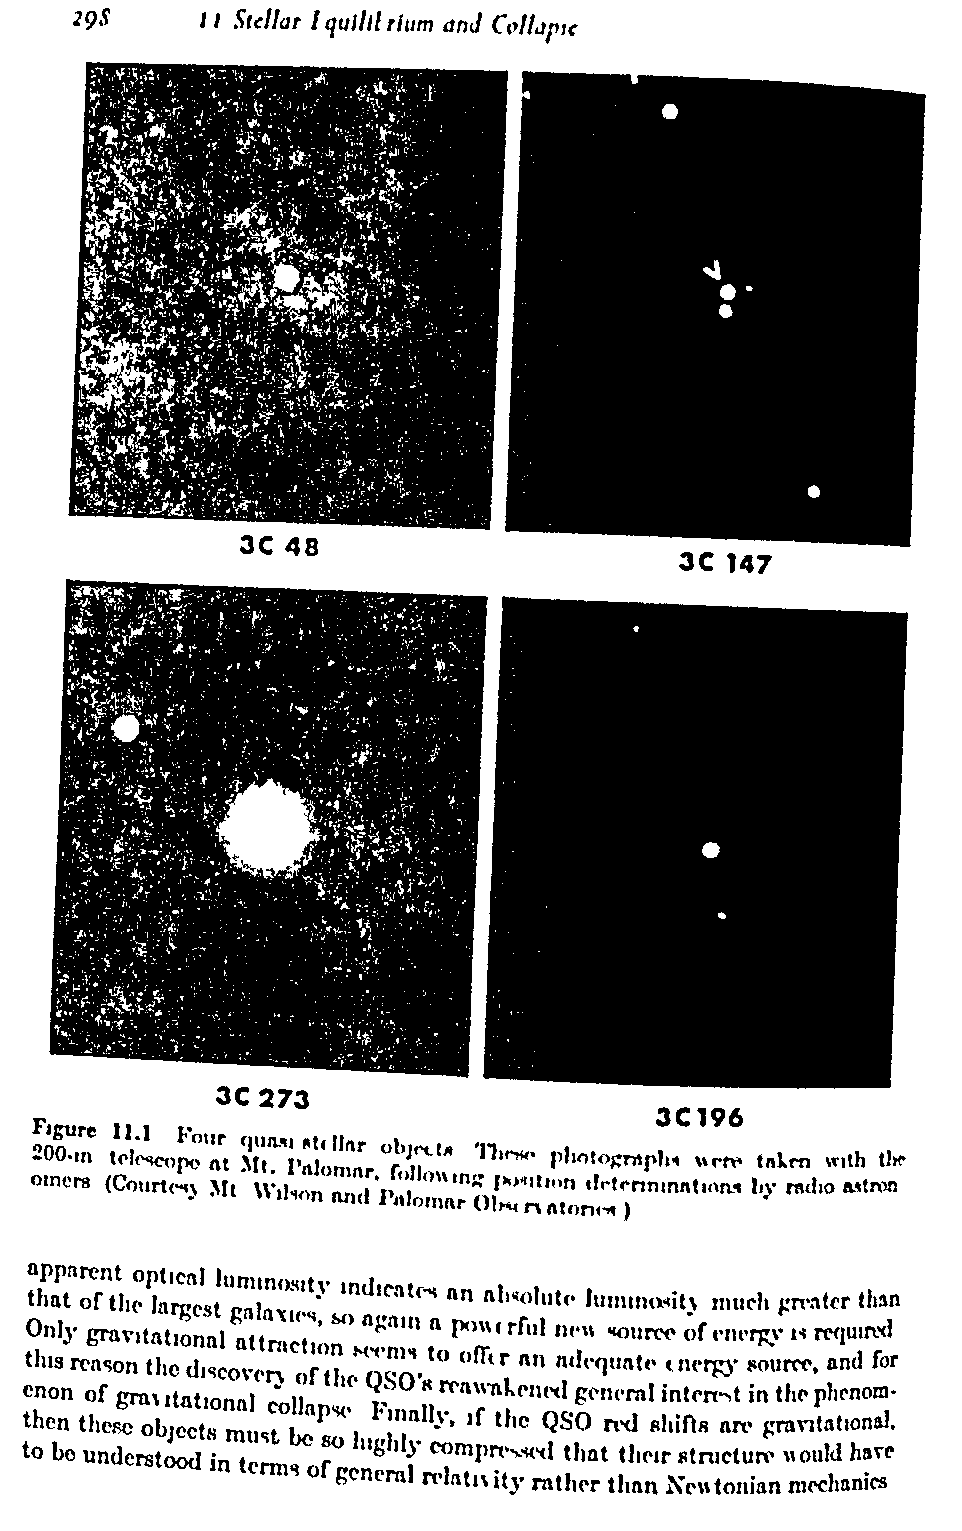
\includegraphics[
      height=0.255\textheight,
      trim=492bp 430bp 44bp 586bp,
      clip
    ]{figures/chapter11/fig11-01-source.png}
    \\
    \small\bfseries 3C 273 & \small\bfseries 3C 196
  \end{tabular}
  \caption{Four quasi-stellar objects. These photographs were taken with the
  200-in.\ telescope at Mt.\ Palomar, following position determinations by
  radio astronomers. (Courtesy Mt.\ Wilson and Palomar Observatories.)}
  \label{fig:11.1}
\end{figure}
\endgroup
